\documentclass[11pt,a4paper]{article}
\usepackage[utf8]{inputenc}
\usepackage[T1]{fontenc}
\usepackage[margin=1in]{geometry}
\usepackage{graphicx}
\usepackage{hyperref}
\usepackage{xcolor}
\usepackage{float}
\usepackage{listings}
\usepackage{upquote}
\usepackage{amsmath}

\lstset{
    basicstyle=\ttfamily\small,
    breaklines=true,
    frame=single,
    numbers=left,
    numberstyle=\tiny,
    backgroundcolor=\color{gray!10},
    keywordstyle=\color{blue},
    commentstyle=\color{green!50!black},
    stringstyle=\color{red},
    showstringspaces=false
}

\title{\textbf{Practice 3 -- Visual Servoing}}
\author{
    Robotics and Cyber-Physical Systems \\
    School of Sciences and Engineering \\
    Tecnol\'ogico de Monterrey
}
\date{}

\begin{document}

\maketitle

\section*{Introduction}

In this practice, you will use the Stretch head cameras to find and follow a
colored object. You will begin by driving the robot manually while observing
its RGB and depth images. You will then add scanning, color segmentation,
visual servoing, depth measurement, and automatic distance control.

Each part starts from the previous one. Keep each completed script so you can
compare how the controller develops.

\subsection*{Before You Begin}

Open a terminal in the repository and update your copy:

\begin{lstlisting}[language=bash]
git pull
uv sync
\end{lstlisting}

If you have uncommitted work, save or commit it before pulling. All robot
movement in this activity must run with collision management enabled, as it is
in \texttt{teleop\_boilerplate.py}.

\newpage

\section*{Part 1 -- Explore with the Head Cameras}

\subsection*{Objective}

Add the head RGB and depth feeds to the teleoperation boilerplate, then use
them to explore the robot's environment.

\subsection*{Background}

\texttt{OpenCV} (imported as \texttt{cv2}) provides tools for displaying and
processing images. \texttt{NumPy} provides efficient numerical arrays; camera
images are represented as NumPy arrays of pixel values.

\subsection*{Task}

Copy the boilerplate:

\begin{lstlisting}[language=bash]
cp teleop_boilerplate.py p3_1_camera.py
\end{lstlisting}

Add the camera imports:

\begin{lstlisting}[language=Python]
import cv2

from stretch_tools import Cameras, HEAD_CAMERA
\end{lstlisting}

Create the camera interface after creating the teleoperation objects:

\begin{lstlisting}[language=Python]
cameras = Cameras(head_info=HEAD_CAMERA)
\end{lstlisting}

Inside the loop, read and display both head feeds:

\begin{lstlisting}[language=Python]
success, frame, depth_frame = cameras.read_head()
if success:
    cv2.imshow("Head RGB", frame)
    cv2.imshow("Head Depth", depth_frame)

if cv2.waitKey(1) & 0xFF == ord("q"):
    break
\end{lstlisting}

Finally, close the cameras and windows in the \texttt{finally} block:

\begin{lstlisting}[language=Python]
cameras.close()
cv2.destroyAllWindows()
\end{lstlisting}

Run the program with \texttt{uv run p3\_1\_camera.py}. Press \texttt{h} to
switch the keyboard controls to the head, then use \texttt{I}, \texttt{J},
\texttt{K}, and \texttt{L} to look around. Drive carefully and observe how
objects appear in both images.

\begin{figure}[H]
    \centering
    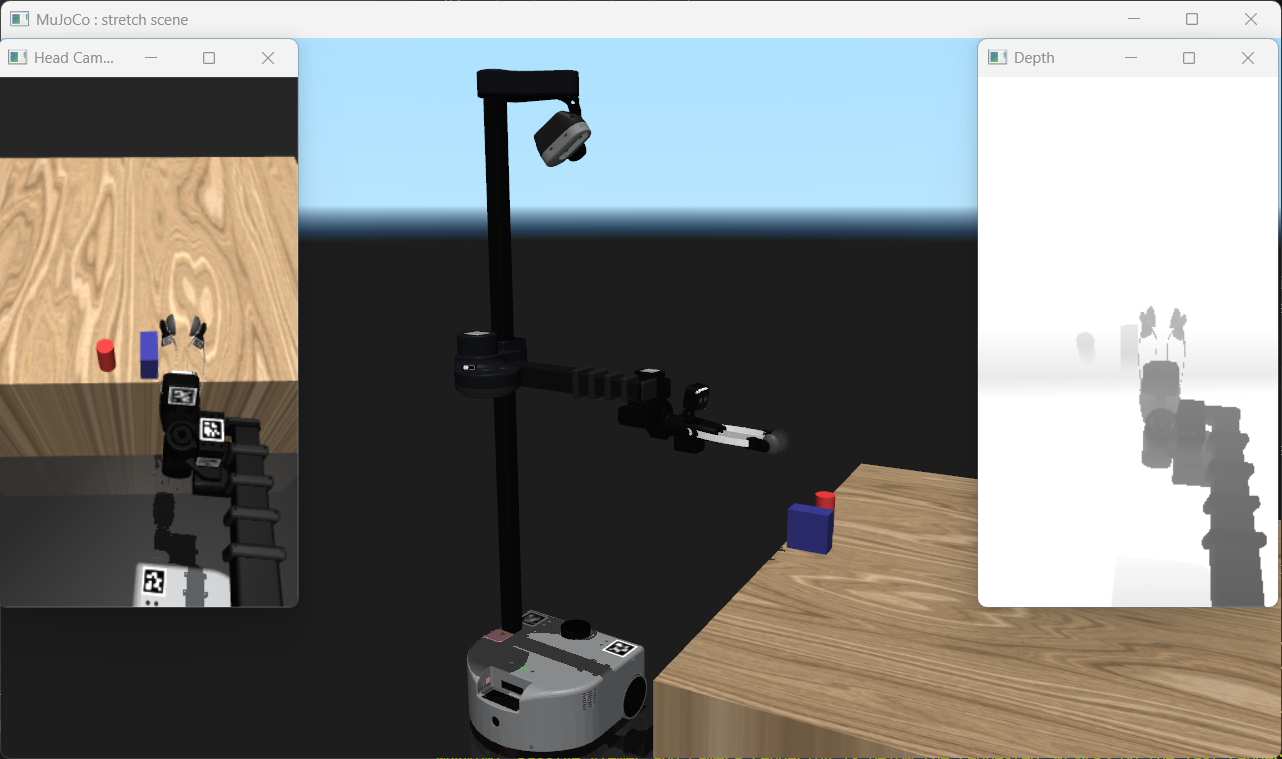
\includegraphics[width=0.8\textwidth]{p3_1_cameras.png}
    \caption{The head RGB and depth camera feeds.}
\end{figure}

\newpage

\section*{Part 2 -- Scan the Environment}

\subsection*{Objective}

Make the robot rotate while keeping its head in a useful scanning pose.

\subsection*{Background}

A \texttt{StateController} converts a desired joint position into velocity
commands. It continues correcting the joint if it is disturbed, so it is more
useful here than issuing a position command only once.

\subsection*{Task}

Copy Part 1 to \texttt{p3\_2\_scan.py}. Import \texttt{math} and
\texttt{StateController}, then create the scanning state:

\begin{lstlisting}[language=Python]
scanning_position = StateController(
    stretch,
    {
        "head_pan_counterclockwise": 0.0,
        "head_tilt_up": math.radians(-30),
    },
)
\end{lstlisting}

At the beginning of each loop, request the scanning pose and add a slow base
rotation:

\begin{lstlisting}[language=Python]
command = scanning_position.get_command()
command["base_counterclockwise"] = -0.3
command = teleop.get_manual_override(command)
controller.set_command(command)
\end{lstlisting}

The robot should rotate continuously while keeping the head facing forward
and pitched down. Manual input can still override the autonomous command.

\newpage

\section*{Part 3 -- Detect a Red Object}

\subsection*{Objective}

Create an HSV mask, find the largest red region, and print its image position.

\subsection*{Task}

Copy Part 2 to \texttt{p3\_3\_detection.py} and import NumPy:

\begin{lstlisting}[language=Python]
import numpy as np
\end{lstlisting}

Red wraps around the beginning and end of OpenCV's hue range, so it requires
two ranges:

\begin{lstlisting}[language=Python]
lower_1 = np.array([0, 100, 100])
upper_1 = np.array([10, 255, 255])
lower_2 = np.array([170, 100, 100])
upper_2 = np.array([179, 255, 255])
\end{lstlisting}

Inside the camera block, create and display the mask:

\begin{lstlisting}[language=Python]
hsv = cv2.cvtColor(frame, cv2.COLOR_BGR2HSV)
mask = cv2.inRange(hsv, lower_1, upper_1)
mask |= cv2.inRange(hsv, lower_2, upper_2)
cv2.imshow("Red Mask", mask)
\end{lstlisting}

Use \texttt{cv2.findContours()}, select the largest contour, and use
\texttt{cv2.moments()} to calculate its center:

\begin{lstlisting}[language=Python]
contours, _ = cv2.findContours(
    mask, cv2.RETR_EXTERNAL, cv2.CHAIN_APPROX_SIMPLE
)
if contours:
    contour = max(contours, key=cv2.contourArea)
    moments = cv2.moments(contour)
    if cv2.contourArea(contour) > 100 and moments["m00"]:
        x = int(moments["m10"] / moments["m00"])
        y = int(moments["m01"] / moments["m00"])
        print(x, y)
\end{lstlisting}

Move the object through the image and observe how its printed pixel position
changes.

\begin{figure}[H]
    \centering
    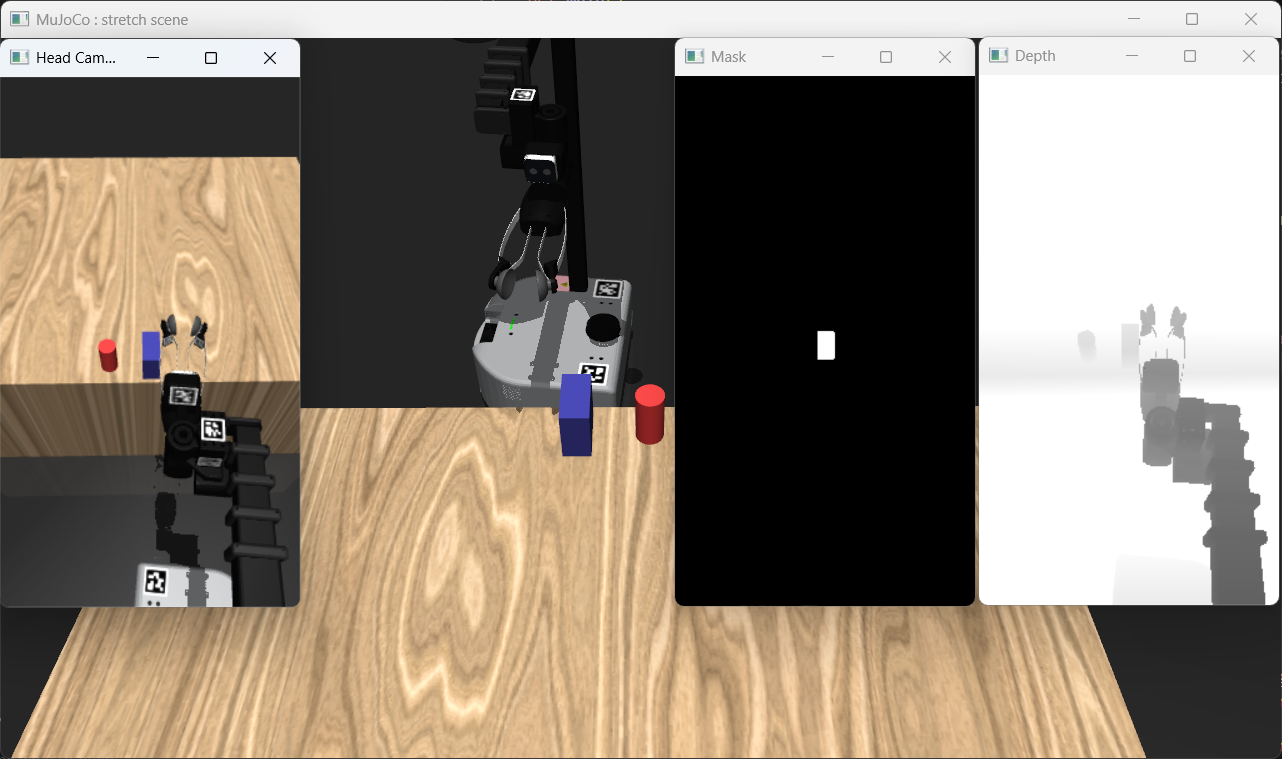
\includegraphics[width=0.8\textwidth]{p3_3_mask.png}
    \caption{The RGB, depth, and wrapped-red mask windows.}
\end{figure}

\newpage

\section*{Part 4 -- Follow the Object}

\subsection*{Objective}

Refactor object detection into a function, then use proportional control to
turn the base and tilt the head toward the object.

\subsection*{Task}

Copy Part 3 to \texttt{p3\_4\_servo.py}. Move the masking and centroid logic
into a function:

\begin{lstlisting}[language=Python]
def detect_object(frame):
    # Create the wrapped-red mask and find its largest contour.
    # Return (x, y) when the contour is valid.
    # Return None when no object is found.
\end{lstlisting}

The function should return only the object's center. The mask window is no
longer needed.

Create a second state controller that holds head pan at zero:

\begin{lstlisting}[language=Python]
head_forward = StateController(
    stretch,
    {"head_pan_counterclockwise": 0.0},
)
\end{lstlisting}

When the object is visible, normalize its offset from the image center and
generate commands:

\begin{lstlisting}[language=Python]
KP = 0.5

x, y = center
height, width = frame.shape[:2]
horizontal_error = (x - width / 2) / (width / 2)
vertical_error = (y - height / 2) / (height / 2)

command = head_forward.get_command()
command["base_counterclockwise"] = -KP * horizontal_error
command["head_tilt_up"] = -KP * vertical_error
\end{lstlisting}

This is proportional control: \textbf{the further away the object is from the
center, the harder the robot will turn toward it}. As the object approaches
the center, the command naturally becomes smaller. The base handles horizontal
alignment while the head remains pointed forward; head tilt handles vertical
alignment.

\begin{figure}[H]
    \centering
    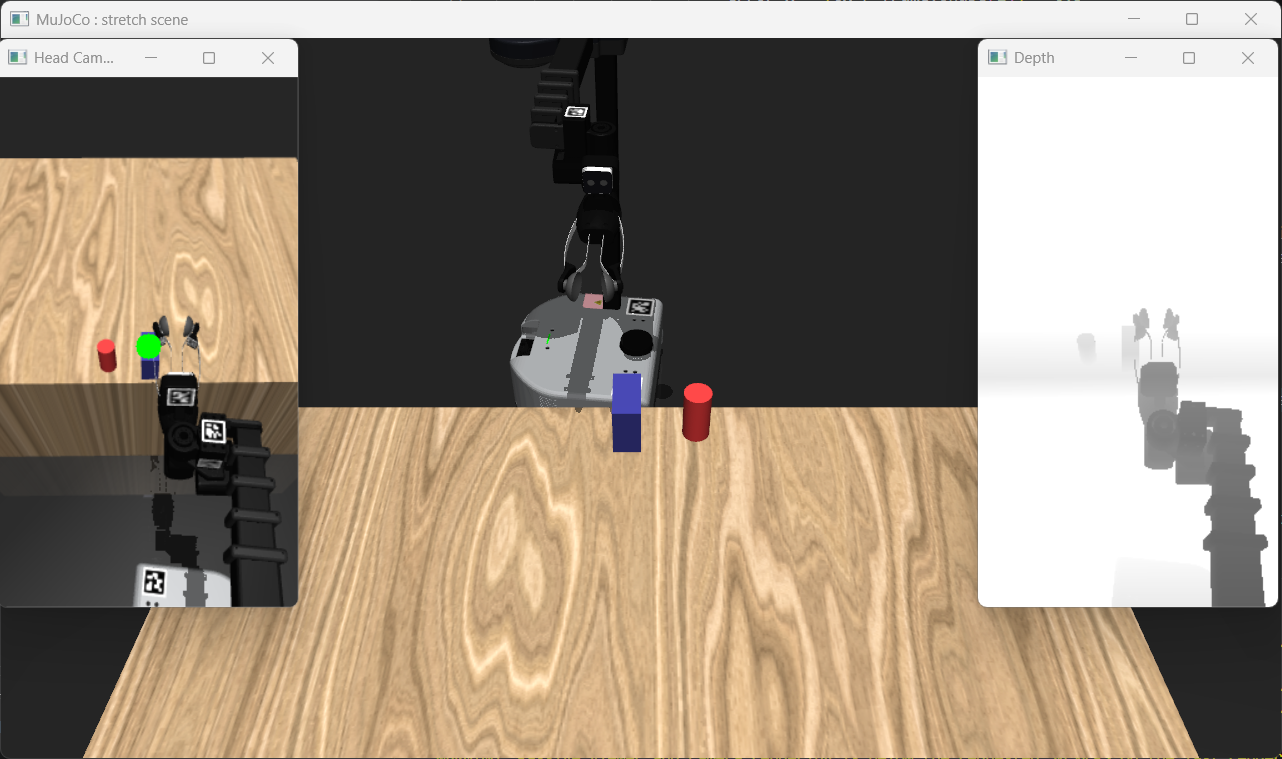
\includegraphics[width=0.8\textwidth]{p3_4_servo.png}
    \caption{The robot turning to keep the detected object centered.}
\end{figure}

\newpage

\section*{Part 5 -- Measure Distance}

\subsection*{Objective}

Use the head depth image to measure the distance to the detected object.

\subsection*{Background}

The depth image stores a distance measurement at each pixel. A value of zero
usually means that no valid measurement was available. The public
\texttt{Cameras} interface represents depth in millimetres, while
\texttt{HEAD\_CAMERA.get\_depth()} converts the measurement to metres and
accounts for the different RGB and depth camera intrinsics.

\subsection*{Task}

Copy Part 4 to \texttt{p3\_5\_depth.py}. Read both frames together, then look
up the depth at the detected RGB position:

\begin{lstlisting}[language=Python]
success, frame, depth_frame = cameras.read_head()

center = detect_object(frame)
if center:
    distance = HEAD_CAMERA.get_depth(center, depth_frame)
    if distance is not None:
        print(f"Distance: {distance:.3f} m")
\end{lstlisting}

Move the object closer and farther away and compare the physical distance with
the printed value.

\newpage

\section*{Part 6 -- Approach the Object}

\subsection*{Objective}

Make the robot approach or retreat from the object until it is approximately
\(0.75\) metres away.

\subsection*{Task}

Copy Part 5 to \texttt{p3\_6\_distance\_control.py} and add:

\begin{lstlisting}[language=Python]
KP_DISTANCE = 10.0
TARGET_DISTANCE = 0.75
\end{lstlisting}

Calculate the distance error and the horizontal alignment factor:

\begin{lstlisting}[language=Python]
distance_error = distance - TARGET_DISTANCE
alignment = 1.0 - abs(horizontal_error)

command["base_forward"] = alignment * np.clip(
    KP_DISTANCE * distance_error, -1.0, 1.0
)
\end{lstlisting}

Set \texttt{base\_forward} to zero whenever the object or its depth is not
available.

The \textbf{alignment factor is essential}. When the object is near the edge
of the image, the factor approaches zero and the robot prioritizes rotation.
As the object becomes centered, the factor approaches one and grants the
distance controller more authority to drive forward or backward. Without this
factor, the robot could move strongly toward an object before it is actually
facing it.

Test the controller from several starting angles and distances. The robot
should first face the object, then settle close to the target distance while
continuing to track it vertically.

\newpage

\section*{Deliverable}

Submit your six Python scripts and a short video demonstrating Part 6. The
video should show the robot finding the red object, rotating to face it,
approaching or retreating, and settling near \(0.75\) metres. Briefly explain
HSV masking, proportional visual error, depth measurement, and the purpose of
the alignment factor.

\end{document}
